\headline{{\textbf{\Large\sffamily Potting Shed Gossip:}}\\
          {\textbf{\large\sffamily Twickenham Takes On the New Talent Challenge}}}
\label{2025-06-gossip}
\noindent
This month, two of our own---David Fishwick and Mark Pittman---stepped onto the national stage at the Federation of British Bonsai Societies (FoBBS) New Talent Competition, a rigorous contest designed to spotlight emerging bonsai artists.

The rules are strict: no professionals, no past winners, and no shortcuts.
Competitors must bring their own tools and wire, while FoBBS provides the tree---a level playing field where skill alone decides the winner.
The prize?
A chance to represent the UK at the European New Talent Final, with travel and accommodation supported by the Federation.

\textit{``It's about raw talent meeting opportunity,''} says David, who prepared for months.
\textit{``You're handed a tree you've never worked on before, and in a few hours, you have to reveal its soul.''}
Mark, equally determined, added: \textit{``The pressure was intense, but just being there felt like a victory.''}

\begin{window}[%
    2,l,%
    \includegraphics[width=1.0\columnwidth]{},%
]
\end{window}
\vspace{-1em}
\begin{window}[%
    2,l,%
    \includegraphics[width=1.0\columnwidth]{},%
]
\end{window}
\columnbreak

The judging was nail-bitingly close.
Ryan Houghton (of the Aka Matsu School of Bonsai and YouTube fame) ultimately took the top spot, but the caliber of all three finalists left even the Chelsea Flower Show judge deliberating for an unusually long time.
\textit{``That says everything,''} Mark reflects.
\textit{‘‘When the judge hesitates, you know the work is good.''}

Though our club didn't bring home the trophy this year, David and Mark's participation is a testament to the growing strength of Twickenham's bonsai community.
Their journey reminds us that competitions aren't just about winning---they're about learning, pushing boundaries, and celebrating how far we've come.

\vspace{0.25em}
\begin{center}
    $\cdots$
\end{center}
\vspace{-0.5em}

\noindent
\textit{Inspired to take on the challenge next year?}
\textit{Discuss it at our next meeting---we'd love to cheer on more Twickenham talent!}
\closearticle

\end{multicols}

\begin{center}
\begin{minipage}[b]{0.98\textwidth}
    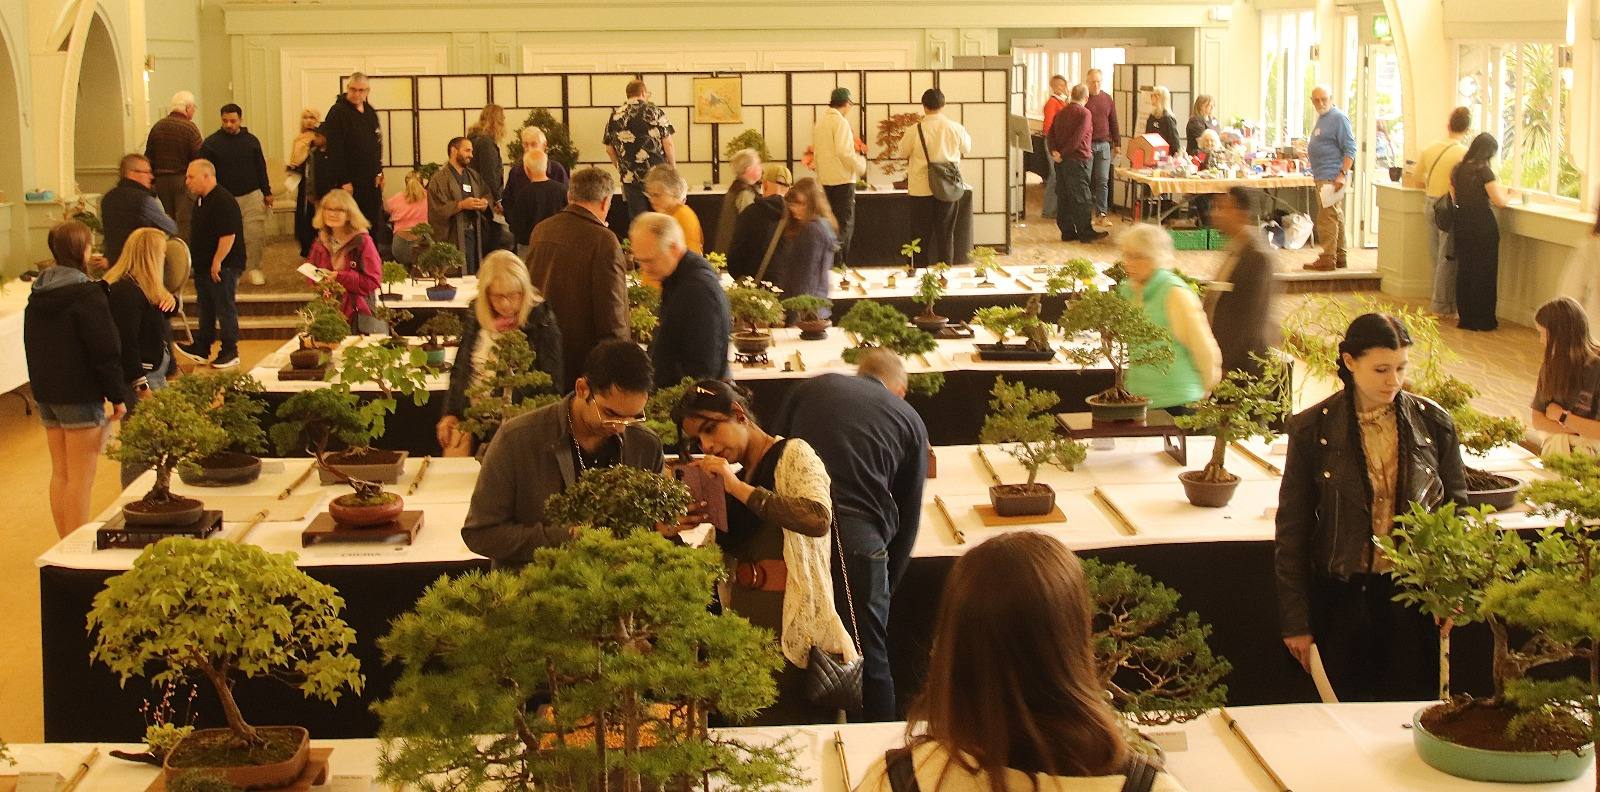
\includegraphics[width=1.0\textwidth]{2025_06/res/gossip_00}
\end{minipage}

\medskip
\begin{minipage}[b]{0.4\textwidth}
    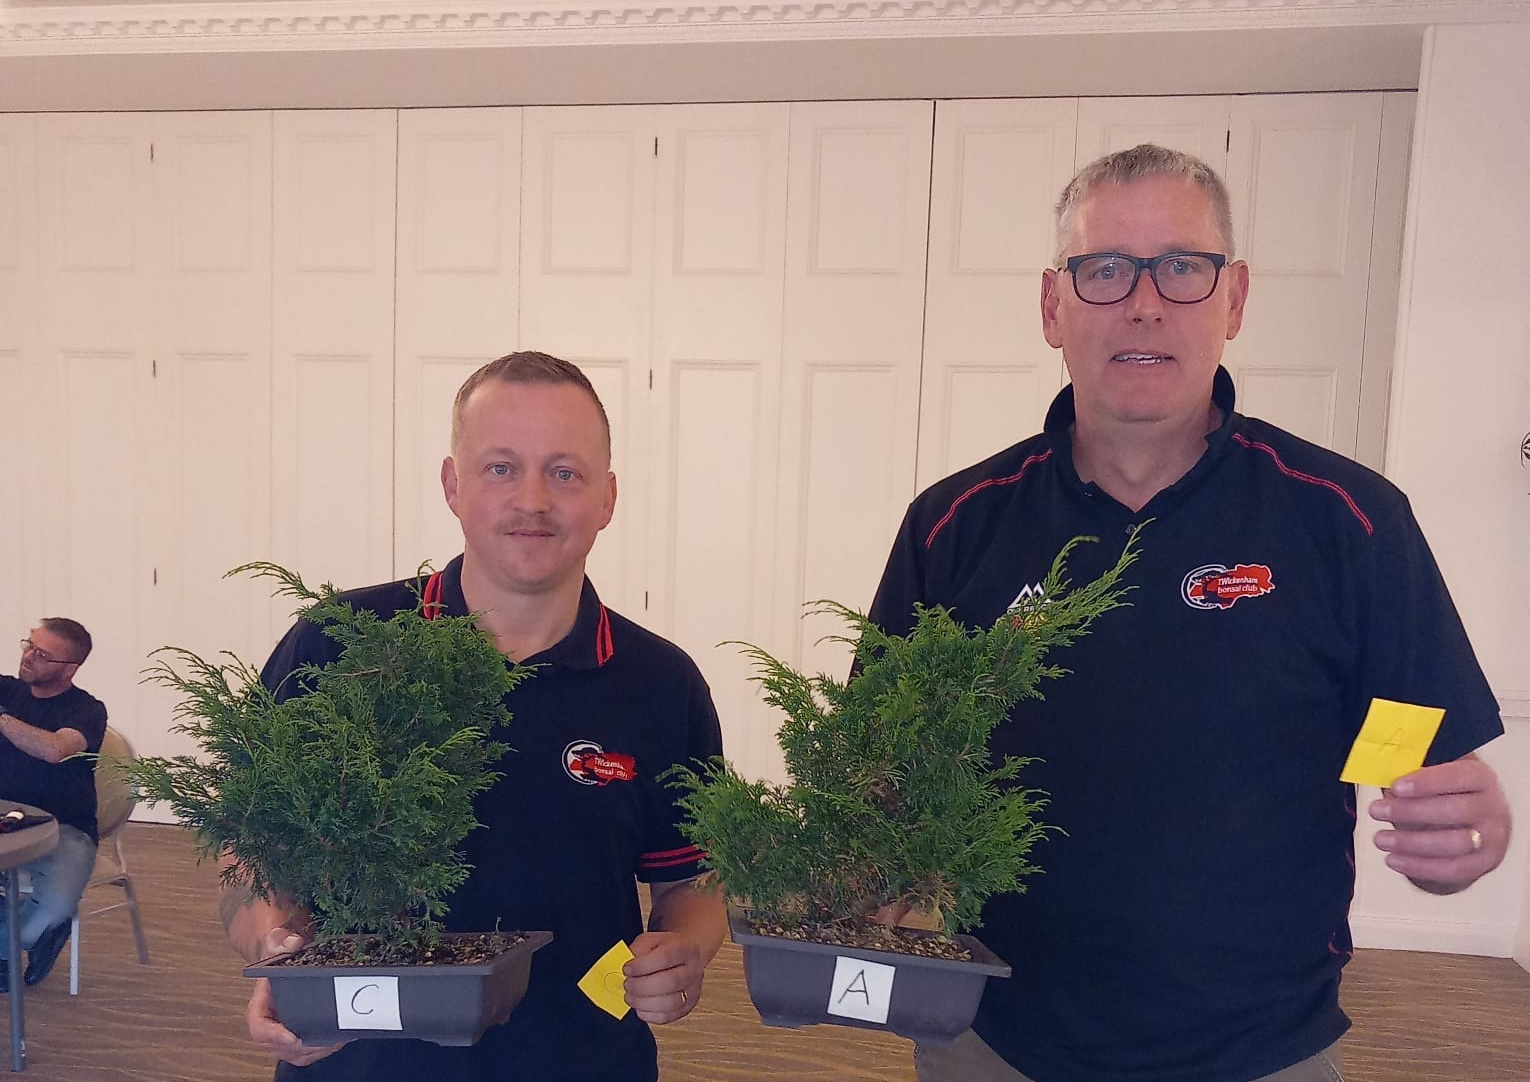
\includegraphics[width=1.0\textwidth]{2025_06/res/gossip_01}
\end{minipage}\qquad
\begin{minipage}[b]{0.27\textwidth}
    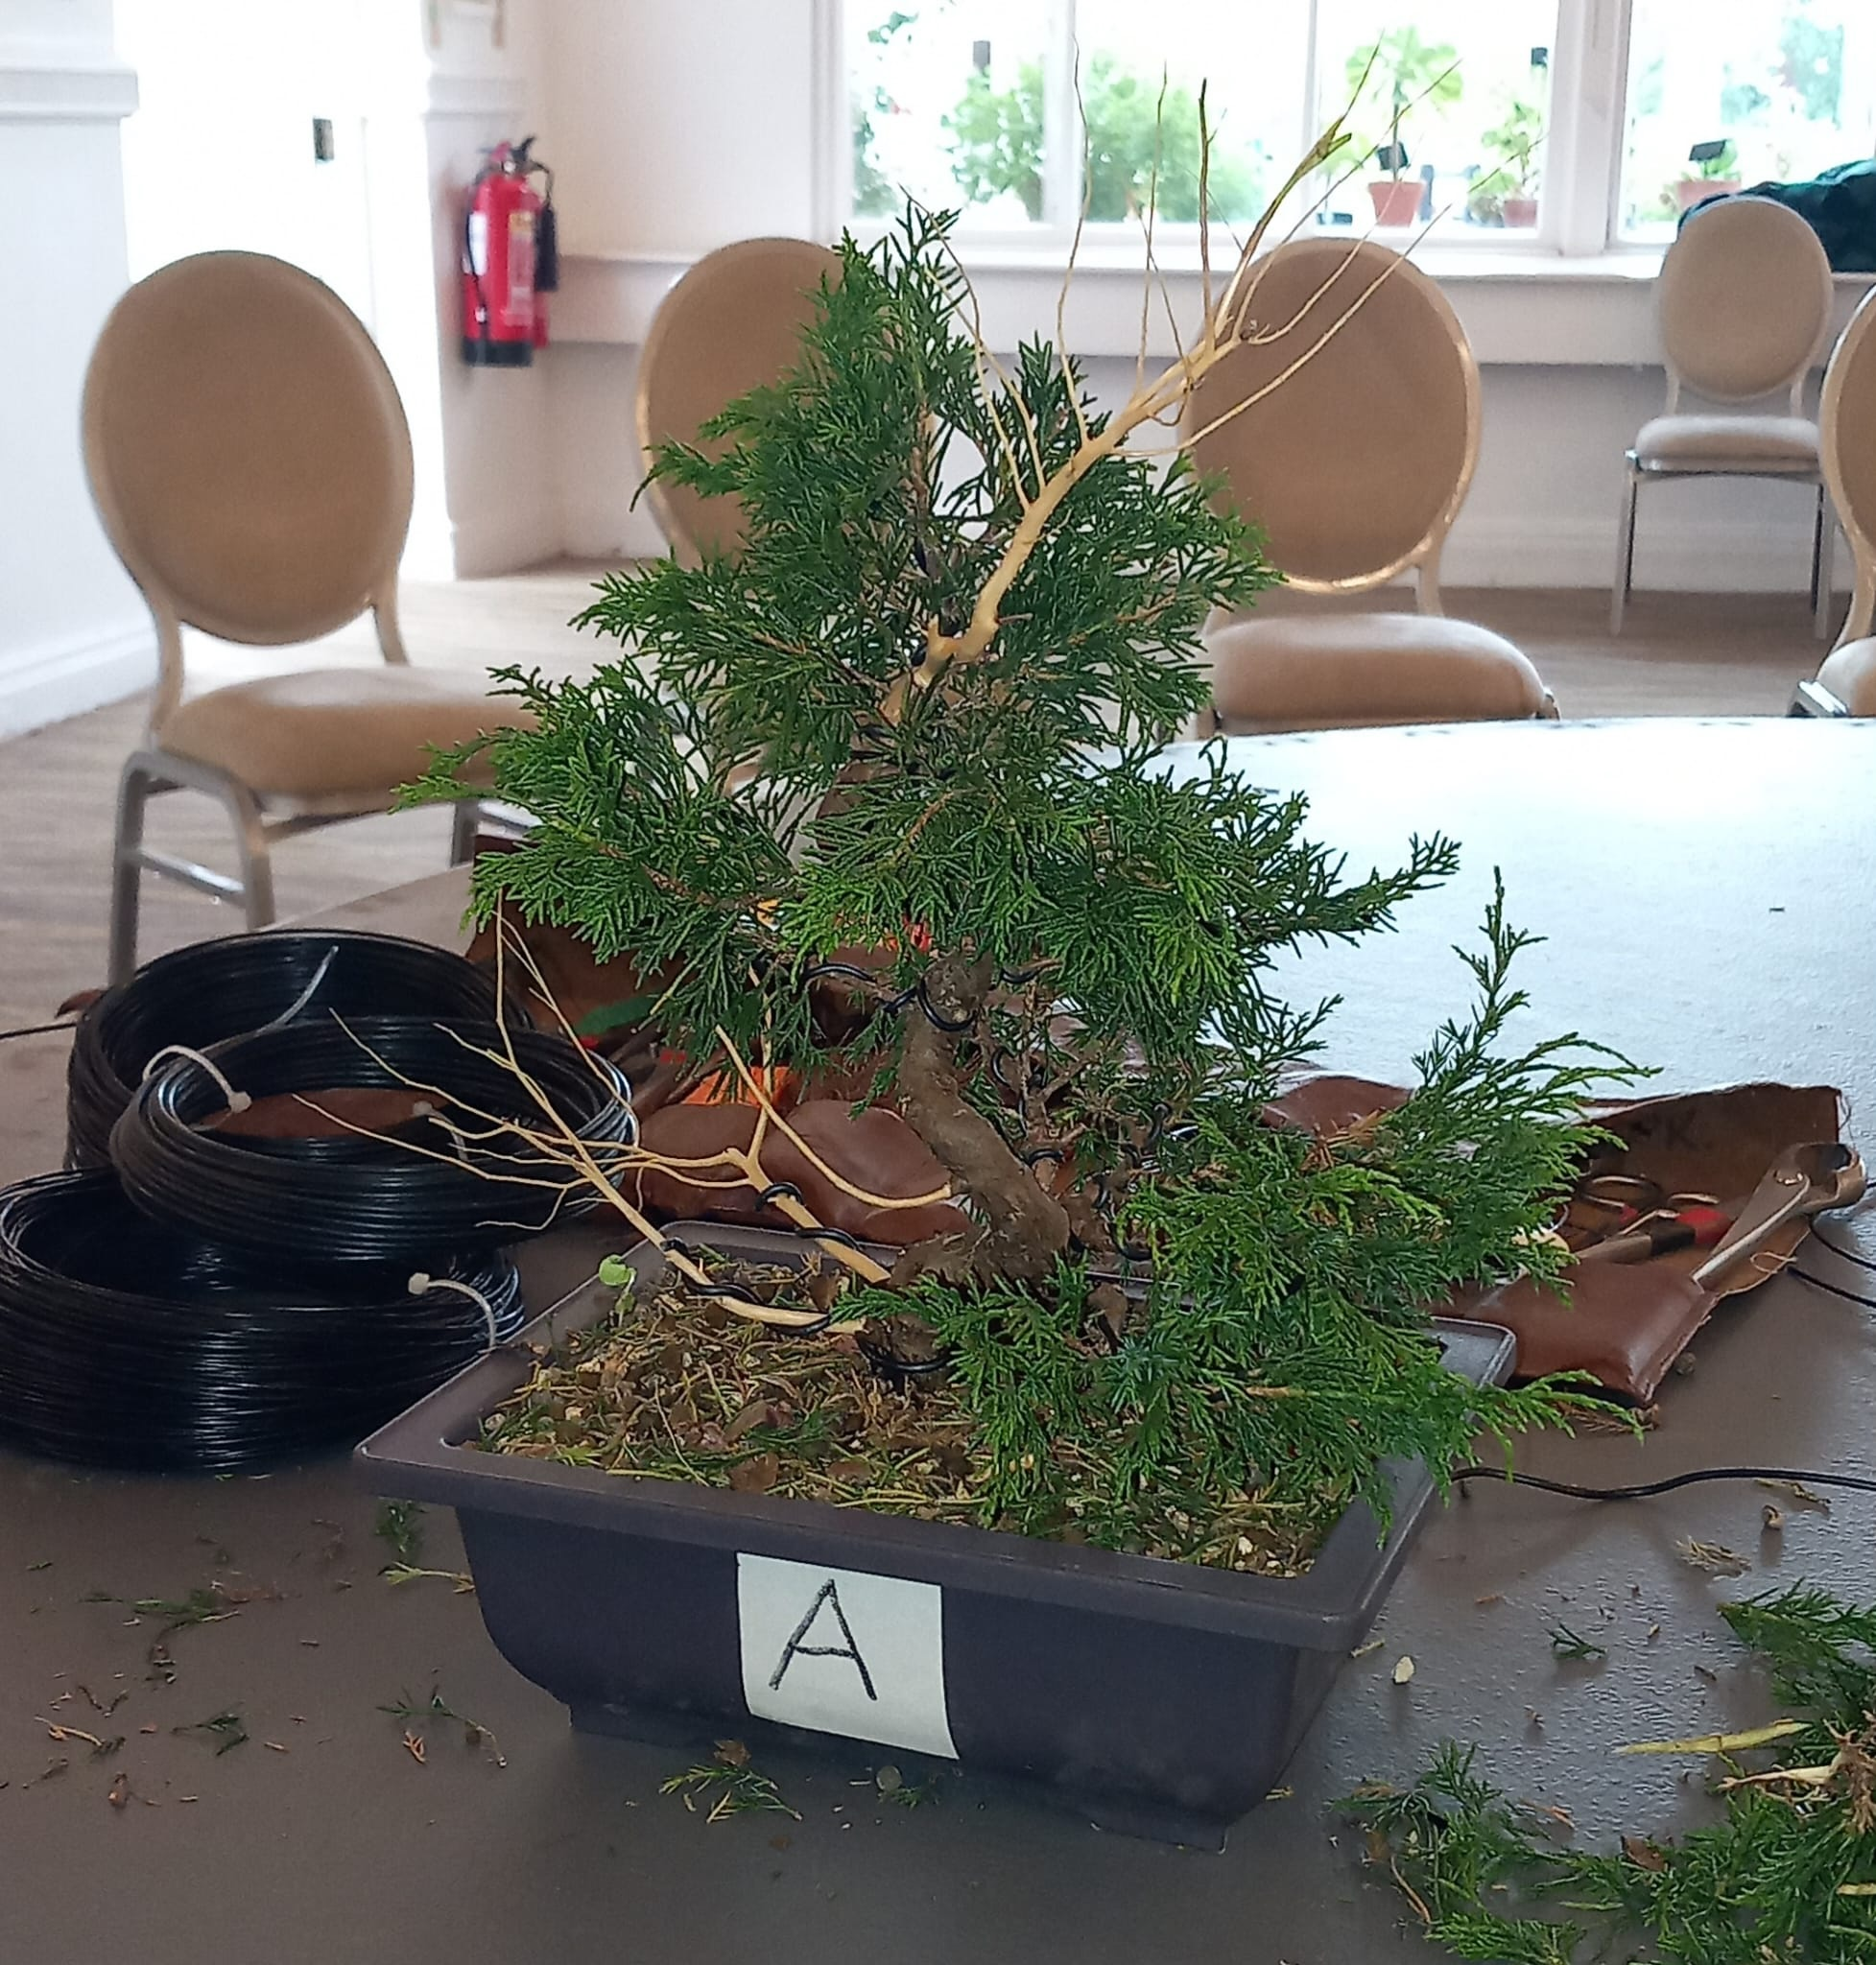
\includegraphics[width=1.0\textwidth]{2025_06/res/gossip_02}
\end{minipage}\qquad
\begin{minipage}[b]{0.23\textwidth}
    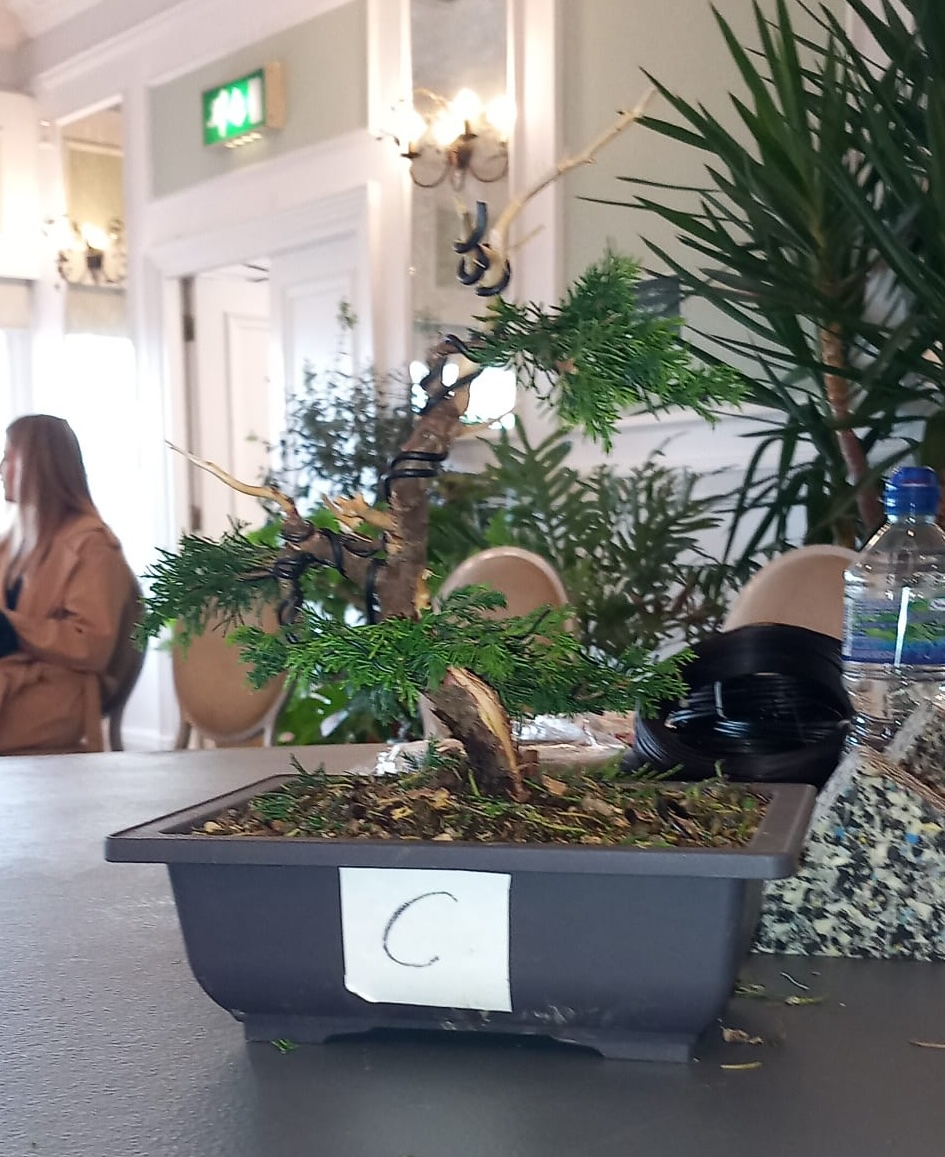
\includegraphics[width=1.0\textwidth]{2025_06/res/gossip_03}
\end{minipage}

\medskip 
\centerline{\emph{The competition trees: a test of vision and technique.}}
\end{center}

\begin{multicols}{2}
